\documentclass{beamer}
%
% Choose how your presentation looks.
%
% For more themes, color themes and font themes, see:
% http://deic.uab.es/~iblanes/beamer_gallery/index_by_theme.html
%
\mode<presentation>
{
  \usetheme{default}      % or try Darmstadt, Madrid, Warsaw, ...
  \usecolortheme{default} % or try albatross, beaver, crane, ...
  \usefonttheme{default}  % or try serif, structurebold, ...
  \setbeamertemplate{navigation symbols}{}
  \setbeamertemplate{caption}[numbered]
} 

\usepackage[english]{babel}
\usepackage[utf8]{inputenc}
\usepackage[T1]{fontenc}

\usepackage{tikz}

\title[Matrizes]{Álgebra matricial}
\author{MAP 2110 - Diurno}
\institute{IME USP}
\date{5 de maio}

\begin{document}

\begin{frame}
  \titlepage
\end{frame}

% Uncomment these lines for an automatically generated outline.
%\begin{frame}{Outline}
%  \tableofcontents
%\end{frame}


\section{Álgebra matricial}

\begin{frame}{O produto de matrizes}

  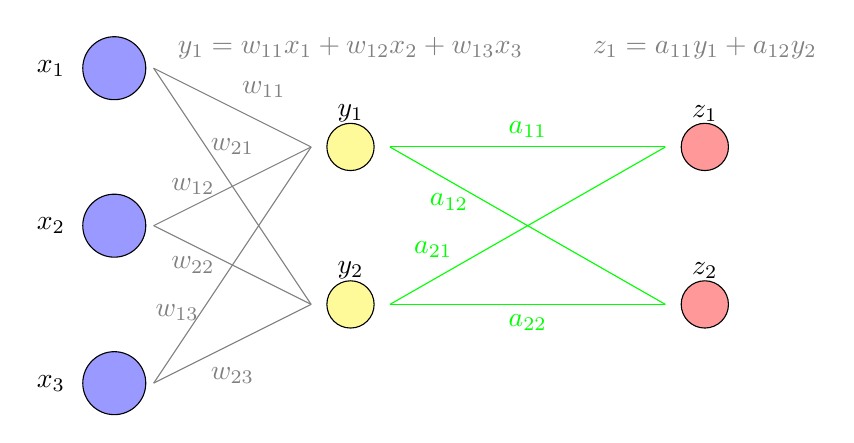
\begin{tikzpicture}
    % primeira parte
    \filldraw[fill=blue!40!white] (0.5,2) circle (0.4cm) node[anchor=east, xshift=-0.5cm] {$x_1$};
    \filldraw[fill=blue!40!white] (0.5,0) circle (0.4cm) node[anchor=east, xshift=-0.5cm] {$x_2$};
    \filldraw[fill=blue!40!white] (0.5,-2) circle (0.4cm) node[anchor=east, xshift=-0.5cm] {$x_3$};
    %segunda parte 
    \filldraw[fill=yellow!40!white] (3.5,1) circle (0.3cm) node[anchor=south, yshift=0.2cm] {$y_1$} 
      node[anchor=south, yshift=1cm, gray] {$y_1 = w_{11}x_1 + w_{12}x_2+w_{13}x_3$};
    \filldraw[fill=yellow!40!white] (3.5,-1) circle (0.3cm) node[anchor=south, yshift=0.2cm] {$y_2$} ;
    %terceira parte
    \filldraw[fill=red!40!white] (8,1) circle (0.3cm) node[anchor=south, yshift=0.2cm] {$z_1$}
    node[anchor=south, yshift=1cm,gray] {$z_1 = a_{11}y_1+a_{12}y_2$};
    \filldraw[fill=red!40!white] (8,-1) circle (0.3cm) node[anchor=south, yshift=0.2cm] {$z_2$};
    % agora as arestas
    \draw[gray] (1,2) -- node[anchor=south west] {$w_{11}$}  (3,1);
    \draw[gray] (1,2) -- node[yshift=0.5cm] {$w_{21}$} (3,-1);
    \draw[gray] (1,0) -- node[xshift=-0.5cm] {$w_{12}$} (3,1);
    \draw[gray] (1,0) -- node[xshift=-0.5cm] {$w_{22}$} (3,-1);
    \draw[gray] (1,-2) -- node[xshift=-0.7cm, yshift=-0.6cm] {$w_{13}$} (3,1);
    \draw[gray] (1,-2) -- node[yshift=-0.4cm] {$w_{23}$}(3,-1);
    % ultimas arestas
    \draw[green] (4,1) -- node[anchor=south] {$a_{11}$} (7.5,1);
    \draw[green] (4,1) -- node[xshift=-1cm, yshift=0.3cm] {$a_{12}$} (7.5,-1);
    \draw[green] (4,-1) -- node[xshift=-1.2cm, yshift=-0.3cm] {$a_{21}$} (7.5,1);
    \draw[green] (4,-1) -- node[anchor=north] {$a_{22}$}(7.5,-1);
\end{tikzpicture}
 
\end{frame}

\begin{frame}{}
  \begin{gather*}
    \begin{bmatrix}
      w_{11} & w_{12} & w_{13} \\
      w_{21} & w_{22} & w_{23} 
    \end{bmatrix} \leftrightarrow (x_1, x_2, x_3) \to (y_1, y_2)
    \text{ e } \\ 
    \begin{bmatrix}
      a_{11} & a_{12} \\ a_{21} & a_{22}
    \end{bmatrix} \leftrightarrow (y_1, y_2) \to (z_1,z_2) \\
    \text{Como seria a matriz de }
    (x_1, x_2 , x_3) \leftrightarrow (z_1, z_2)
\end{gather*}

  
\end{frame}

\begin{frame}{}
  Temos:
  \begin{gather*}
    z_1 = c_{11}x_1 + c_{12}x_2 + c_{13}x_3 \\
    z_2 = c_{21}x_1 + c_{22}x_2 + c_{23}x_3 \\
     c_{ij}\text{ deve ser calculado de }\\
    z_1 = a_{11}y_1 + a_{12}y_2 \\
    z_2 = a_{21}y_1 + a_{22}y_2 \\
    \text{ e } \\
    y_1 = w_{11}x_1 + w_{12}x_2 + w_{13}x_3 \\
    y_2 = w_{21}x_1 + w_{22}x_2 + w_{23}x_3 
  \end{gather*}
  

\end{frame}

\begin{frame}{Fórmula geral da composição}

  Se $A= [a_{ij}]$ é uma matriz com $m$ linhas e $n$ colunas e
  $B = [b_{kl}]$ é uma matriz com $n$ linhas e $r$ colunas,
  então definimos o produto como a matriz $A.B=C =[c_{il}]$ com $m$ linhas e 
  $r$ colunas, pela Fórmula
  $$ c_{il} = \sum_{p=1}^{n}a_{ip}b_{pl} $$
  

  
\end{frame}


\begin{frame}{ }
 
  $$
\begin{array}{|c|ccc|ccc|} \hline
& & & &  & l &   \\ \hline
& & & & *& b_{1l} & * \\
& & & & * & \vdots & *  \\
& & & & * & b_{nl} & * \\ \hline  
& * & * & * &  & \downarrow & \\
i& a_{i1} & \cdots & a_{in} & \rightarrow & c_{il} & \\
 &* & * & * & & & \\ \hline 
\end{array}
  $$
\end{frame}

\begin{frame}{Exemplo }

  \begin{gather*}
    \begin{bmatrix}
      2 & 1 & 3 \\
      0 & -1 & 2 \\
      5 & 3 & 4 
    \end{bmatrix} . \begin{bmatrix}
      x_1 \\ x_2 \\ x_3
    \end{bmatrix} = \begin{bmatrix}
      2x_1 + x_2 + 3x_3 \\
      -x_2 + 2x_3 \\
      5x_1 + 3x_2 + 4x_3
    \end{bmatrix}= \\
     x_1\begin{bmatrix}
      2 \\ 0 \\ 5 
    \end{bmatrix}+x_2 \begin{bmatrix}
      1 \\ -1 \\ 3 
    \end{bmatrix} +x_3 \begin{bmatrix}
      3 \\ 2 \\ 4
    \end{bmatrix} 
  \end{gather*}

\end{frame}

\begin{frame}

Como resolver a equação

\begin{gather*}
\begin{bmatrix}
  2& -1 &1 \\
  1 & 0 & 1  
\end{bmatrix} A = \begin{bmatrix}
  2 & 0 \\ 1 & 2
\end{bmatrix}
  \end{gather*}

\end{frame}

\begin{frame}{Como antes}
\begin{gather*}
 \begin{array}{ccc|cc}
  2& -1 &1 & 2 & 0 \\
  1 & 0 & 1& 1 & 2
 \end{array} \rightarrow \begin{array}{ccc|cc}
  2& -1 &1 & 2 & 0 \\
  0 & 1/2 & 1/2 & 0 & 2
 \end{array} \rightarrow \begin{array}{ccc|cc}
  2& -1 &1 & 2 & 0 \\
  0 & 1 & 1& 0 & 4
 \end{array} \\
 \rightarrow \begin{array}{ccc|cc}
  2& 0 &2 & 2 & 4 \\
  0 & 1 & 1& 0 & 4
 \end{array} \rightarrow \begin{array}{ccc|cc}
  1& 0 &1 & 1 & 2 \\
  0 & 1 & 1& 0 & 4
 \end{array}
\end{gather*}
 \end{frame}

\begin{frame}
$$
\begin{array}{|ccc|cc|} \hline
  & & & a_{11} & a_{12} \\ 
  & & & a_{21} & a_{22} \\ 
  & & & a_{31} (t) & a_{32} (s)\\ \hline
  1& 0 &1 & 1 & 2 \\
  0 & 1 & 1& 0 & 4 \\ \hline
  \end{array}
$$\pause 
$$ A = \begin{bmatrix}
  1-t & 2-s\\
  -t & 4-s\\
  t & s
\end{bmatrix} $$
\end{frame}
\begin{frame}
  
\end{frame}


\begin{frame}{matriz identidade}

A matriz identidade de dimensão $n$ é a matriz $I =[\delta_{ij}]$ com $n$
linhas e $n$ colunas que $\delta_{ii} =1$ para todo $i$ e $\delta_{ij}=0$ quando
$i$ e $j$ são diferentes. No caso de dimensão $3$
\begin{gather*}
  I = \begin{bmatrix}
    1 & 0 & 0 \\ 0 & 1 & 0 \\ 0 & 0 & 1 
  \end{bmatrix}
\end{gather*}
   Note que sempre teremos $I.A= A$ se o número de linhas de $A$ for o mesmo que a dimensão de $I$ e
   $B.I=B$ se o número de colunas de $B$ for igual à dimensão de $I$

   Faremos as contas só para o primeiro caso:
   $A=[a_{ij}]$ com $i\in \{1,\dots,n\}$ e $j\in \{1,\dots, r\}$ e temos $I=[\delta_{ij}]$ $1 \leq i,j \leq n$.

   Então $I.A= [c_{ij}]$ pode-se escrever como:
   \begin{gather*}
     c_{ij} = \sum_{k=1}^n \delta_{ik}a_{kj} = a_{ij}
   \end{gather*}
   pois $\delta_{ik}$ só é diferente de zero quando $k=i$.

 \end{frame}

 \begin{frame}
   
 \end{frame}



\begin{frame}{ Matrizes Elementares }
Lembrando das três operações elementares nas linhas:
\begin{itemize}
  \item $L_1$ trocar duas linhas
  \item $L_2$ multiplicar uma linha por um fator $\alpha$ não nulo.
  \item $L_3$ substituir uma linha, por esta mais o multiplo de uma outra linha.
\end{itemize}
Quando realizamos uma operação elementar na matriz indentidade
 obtemos uma matriz elementar.
 Exemplos de matrizes elementares
\begin{gather*}
  \begin{bmatrix}
    0 & 1 & 0 \\
    1 & 0 & 0 \\
    0 & 0 & 1 
  \end{bmatrix} \begin{bmatrix}
    1 & 0 & 0 \\
    0 & 2 & 0 \\
    0 & 0 & 1 
  \end{bmatrix}\begin{bmatrix}
    1 & 0 & 0 \\
    2 & 1 & 0 \\
    0 & 0 & 1 
  \end{bmatrix}
\end{gather*}
\end{frame}
\begin{frame}{Exercício}
 Calcular os produtos:
 \begin{gather*}
  \begin{bmatrix}
    0 & 1 & 0 \\
    1 & 0 & 0 \\
    0 & 0 & 1 
  \end{bmatrix}. \begin{bmatrix}
    a_{11} & a_{12} & a_{13} \\
    a_{21} & a_{22} & a_{23} \\
    a_{31} & a_{32} & a_{33}
  \end{bmatrix} \text{ e }\begin{bmatrix}
    1 & 0 & 0 \\
    0 & 1 & 0 \\
    0 & 2 & 1 
  \end{bmatrix}. \begin{bmatrix}
    a_{11} & a_{12} & a_{13} \\
    a_{21} & a_{22} & a_{23} \\
    a_{31} & a_{32} & a_{33}
  \end{bmatrix} 
  \end{gather*}
  resposta : \pause 

  \textcolor{red}{
    \begin{gather*}
    \begin{bmatrix}
      a_{21} & a_{22} & a_{23} \\
      a_{11} & a_{12} & a_{13} \\
      a_{31} & a_{32} & a_{33}
    \end{bmatrix} \text{ e }\begin{bmatrix}
      a_{11} & a_{12} & a_{13} \\
      a_{21} & a_{22} & a_{23} \\
      a_{31} + 2a_{21} & a_{32} +2a_{22} & a_{33} +2a_{23}
    \end{bmatrix} 
  \end{gather*}
  }
\end{frame}

\begin{frame}
  
\end{frame}


\begin{frame}{Verdadeiro ou Falso}
  \begin{block}{1}
  A matriz 
  $$ \begin{pmatrix}
    1 & 2 & 3 \\ 
    0 & 1 & 1 \\
    0 & 1 & 1
  \end{pmatrix}$$ tem posto $2$
\end{block}
\end{frame}

\begin{frame}{Verdadeiro ou Falso}
  \begin{block}{2}
  A matriz 
  $$ \begin{pmatrix}
    1 & 2 & 3 \\ 
    0 & 1 & 1 \\
    0 & 1 & 2
  \end{pmatrix}$$ tem posto $2$
\end{block}
\end{frame}

\begin{frame}{Verdadeiro ou Falso}
  \begin{block}{3}
  O sistema linear 
  \begin{gather*}
    a_{11}x_1 + a_{12}x_2 = 0 \\
    a_{21}x_1 + a_{22}x_2 = 0 \\
    a_{31}x_1 + a_{32}x_2 = 0
  \end{gather*} pode não ter nenhuma solução, dependendo da matriz dos 
  coeficientes $[a_{ij}]$
\end{block}
\end{frame}   

\begin{frame}{Verdadeiro ou Falso}
  \begin{block}{4}
  Num determinado ponto do processo de eliminação de Gauss obtivemos 
  a matriz
  $$ \left[ 
  \begin{array}{cccc|c}
    1 & -1 & 2 & 0 & 3 \\
    0 & 0 & 1  & 2 & 1 \\
    0 & 0 & 0  & 2 & a \\
    0 & 0 & 0 & 1 & b
  \end{array}  
  \right]$$
  Então o sistema terá solução se, e somente se $a=2b$
\end{block}
\end{frame}

\begin{frame}{Verdadeiro ou Falso}
  \begin{block}{5}
  considere o sistema linear
  \begin{gather*}
    a_{11}x_1 + a_{12}x_2  + a_{13}x_3= 1 \\
    a_{21}x_1 + a_{22}x_2  + a_{23}x_3= 2\\
    a_{31}x_1 + a_{32}x_2 + a_{33}x_3= 0
  \end{gather*}
  Então se $(u_1,u_2,u_3)$ e $(v_1,v_2,v_2)$ são duas soluções diferentes então
  $(u_1,u_2,u_3)+ (v_1,v_2,v_3)$ também é solução.
\end{block}
\end{frame}
\begin{frame}{Verdadeiro ou Falso}
  \begin{block}{5}
  considere o sistema linear
  \begin{gather*}
    a_{11}x_1 + a_{12}x_2  + a_{13}x_3= 1 \\
    a_{21}x_1 + a_{22}x_2  + a_{23}x_3= 2\\
    a_{31}x_1 + a_{32}x_2 + a_{33}x_3= 0
  \end{gather*}
  Então se $(u_1,u_2,u_3)$ e $(v_1,v_2,v_2)$ são duas soluções diferentes então
  $\lambda(u_1,u_2,u_3)+ (1-\lambda)(v_1,v_2,v_3)$ também é solução.
\end{block}
\end{frame}


\end{document}
